\documentclass[10pt,serif,mathserif,compress,hyperref={colorlinks}]{beamer}
\mode<presentation>
%\usepackage{times} % pour avoir une belle police avec beamer
\usepackage{pgf}
\usepackage{pgfpages}
\usepackage[T1]{fontenc}
\usepackage[utf8]{inputenc}

\usepackage{lmodern}
\usepackage{lastpage}
\usepackage{comment}
\usepackage{geometry}
\usepackage[most]{tcolorbox}
\tcbuselibrary{skins}
\usepackage{beamerthemesplit}
\usepackage{amsmath, amsfonts, epsfig, xspace}
\usepackage{pstricks,pst-node}
\usepackage{multimedia}
\usepackage{pifont}   % zapf dingbats
\usepackage{marvosym} % MarVoSym dingbats
\usepackage{wasysym}

\usepackage{graphicx}% for including figures
\usepackage{tikz}
\usepackage[tikz]{bclogo}
\usetikzlibrary{positioning,decorations.pathreplacing,arrows}
\usepackage{tikzsymbols}

\setlength{\parindent}{0pt}

%%%%%%%%%%%%%%%%%%  Couleurs %%%%%%%%%%%%%%%%%%%%%%%%%%%
\definecolor{mauve}{rgb}{0.5,0,0.7}
\definecolor{carmin}{rgb}{0.7,0,0}
\definecolor{bleu}{rgb}{0,0,0.7}
\definecolor{marron}{rgb}{0.6,0.35,0}
\definecolor{vert}{rgb}{0,0.5,0}
\definecolor{gris}{rgb}{0.9,0.9,0.9}
\definecolor{no}{rgb}{1,0.9,1}
%%%%%%%%%%%%%%%%%%%%%%%%%%%%%%%%%%%%%%%%%%%%%%%%%%%%%%%%%%

\definecolor{White}        {rgb}{1.0,1.0,1.0}

\definecolor{VeryDarkBlue} {RGB}{0,0,153}
\definecolor{DarkBlue}     {rgb}{0.0,0.0,0.6}
\definecolor{Blue}         {rgb}{0.0,0.0,1.0}
\definecolor{MidBlue}      {rgb}{0.6,0.6,1.0}
\definecolor{LightBlue}    {rgb}{0.8,0.8,1.0}
\definecolor{VeryLightBlue}{rgb}{0.9,0.9,1.0}

\definecolor{Gray}{rgb}{0.7,0.7,0.7}
\definecolor{LightGray}{rgb}{0.94,0.94,0.94}

\definecolor{DarkGreen}{rgb}{0,0.6,0}
\definecolor{MidGreen}{rgb}{0.6,1,0.6}
\definecolor{LightGreen}{rgb}{0.88,1,0.88}
\definecolor{VeryLightGreen}{rgb}{0.9,1,0.9}

\definecolor{Yellow}{rgb}{1,1,0.4}
\definecolor{MidYellow}{rgb}{1,1,0.5}
\definecolor{LightYellow}{rgb}{1,1,0.6}
\definecolor{VeryLightYellow}{rgb}{1,1,0.9}

\definecolor{DarkRed}{rgb}{0.7,0.,0.}
\definecolor{Red}{rgb}{0.8,0.,0.}
\definecolor{LightRed}{rgb}{1,0.8,0.8}
\definecolor{VeryLightRed}{rgb}{1,0.9,0.9}

\definecolor{Mauve}{rgb}{0.7,0.,0.7}

\definecolor{Magenta}{rgb}{1,0.,1}
\definecolor{LightMagenta}{rgb}{1,0.5,1}

\definecolor{Chocolate}{rgb}{0.54,0.2,.004}
\definecolor{DarkChocolate}{RGB}{103,38,.00}

\definecolor{DarkOrange}{rgb}{0.65,0.35,0.}
\definecolor{Orange}{rgb}{.9,0.4,0.}
\definecolor{LightOrange}{rgb}{1,0.8,0.5}

%\definecolor{Brown}{rgb}{0.4,0.4,0.}

\definecolor{LightCyan}{rgb}{0.5,1.,1.}

\definecolor{PBG} {rgb}{1.0,1.0,0.6}
\definecolor{PTXT}{rgb}{0.2,0.2,0.0}
\definecolor{IBG} {rgb}{0.8,0.8,1.0}
\definecolor{ITXT}{rgb}{0.2,0.2,0.0}
\definecolor{OBG} {rgb}{0.8,1.0,0.8}
\definecolor{OTXT}{rgb}{0.0,0.4,0.0}

\newcommand{\CommentVeryLightBlue}[1]{{\textcolor{VeryLightBlue}{#1}}}
\newcommand{\CommentWhite}[1]{{\textcolor{White}{#1}}}

\newcommand{\VeryDarkBlue}[1]{\textcolor{DarkBlue}{#1}}
\newcommand{\DarkBlue}[1]{\textcolor{DarkBlue}{#1}}
\newcommand{\Blue}[1]{\textcolor{Blue}{#1}}
\newcommand{\LightBlue}[1]{\textcolor{LightBlue}{#1}}
\newcommand{\VeryLightBlue}[1]{\textcolor{VeryLightBlue}{#1}}

\newcommand{\DarkGreen}[1]{\textcolor{DarkGreen}{#1}}
\newcommand{\LightGreen}[1]{\textcolor{LightGreen}{#1}}
\newcommand{\VeryLightGreen}[1]{\textcolor{VeryLightGreen}{#1}}
\newcommand{\MidGreen}[1]{\textcolor{MidGreen}{#1}}

\newcommand{\DarkRed}[1]{\textcolor{DarkRed}{#1}}
\newcommand{\Red}[1]{\textcolor{red}{#1}}
\newcommand{\LightRed}[1]{\textcolor{LightRed}{#1}}
\newcommand{\VeryLightRed}[1]{\textcolor{VeryLightRed}{#1}}

\newcommand{\Gray}[1]{\textcolor{gray}{#1}}

\newcommand{\Black}[1]{\textcolor{black}{#1}}

\newcommand{\White}[1]{\textcolor{white}{#1}}

\newcommand{\Mauve}[1]{\textcolor{Mauve}{#1}}

\newcommand{\LightMagenta}[1]{\textcolor{LightMagenta}{#1}}
\newcommand{\Magenta}[1]{\textcolor{Magenta}{#1}}

\newcommand{\DarkOrange}[1]{\textcolor{DarkOrange}{#1}}
\newcommand{\Orange}[1]{\textcolor{Orange}{#1}}
\newcommand{\LightOrange}[1]{\textcolor{LightOrange}{#1}}

\newcommand{\DeepPurple}[1]{{\textcolor[rgb]{0.3,0.,0.6}{#1}}}

\newcommand{\Brown}[1]{{\textcolor{Brown}{#1}}}
\newcommand{\Chocolate}[1]{\textcolor{Chocolate}{#1}}
\newcommand{\DarkChocolate}[1]{\textcolor{DarkChocolate}{#1}}

\definecolor{DBluePy}{RGB}{ 28, 78, 99}
\definecolor{BluePy} {RGB}{ 60,110,131}
\definecolor{MBluePy}{RGB}{200,210,240}
\definecolor{LBluePy}{RGB}{220,230,240}
\definecolor{DOranPy}{RGB}{248,194,  3}
\definecolor{OranPy} {RGB}{255,220, 70}
\definecolor{GreenPy}{RGB}{237,255,204}

\newcommand{\bsh}{\textbackslash}
\newcommand{\bshbsh}{\textbackslash\textbackslash}
\newcommand{\chevrons}{\ttfamily>\hspace*{-0.25mm}>\hspace*{-0.25mm}>\hspace*{0.28mm}\xspace}
\newcommand{\M}[1]{\Mauve{#1}}
\newcommand{\DG}[1]{\DarkGreen{#1}}
\newcommand{\DR}[1]{\DarkRed{#1}}
\newcommand{\B}[1]{\Blue{#1}}
\newcommand{\BPy}[1]{\BluePy{#1}}
\newcommand{\VDB}[1]{\VeryDarkBlue{#1}}
\newcommand{\DO}[1]{\DarkOrange{#1}}
\newcommand{\Or}[1]{\Orange{#1}}
\newcommand{\Choco}[1]{\Chocolate{#1}}
\newcommand*{\truc}{\Gray{\textbullet}}

\newcommand{\bif}[1]{{\ttfamily \M{#1}}}	% Python built in function
\newcommand{\typ}[1]{{\ttfamily \M{#1}}}  % Python built in type
\newcommand{\key}[1]{{\ttfamily \Or{#1}}}
\newcommand{\str}[1]{{\ttfamily \DG{#1}}}
\newcommand{\com}[1]{{\ttfamily \DR{#1}}}
\newcommand{\out}[1]{{\ttfamily \B{#1}}}
\newcommand{\command}[1]{{\ttfamily \Choco{#1}}}
\newcommand{\code}[1]{{\ttfamily \Choco{#1}}}
\newcommand{\file}[1]{{\ttfamily \VDB{#1}}}

\newcommand{\bifBF}[1]{\textbf{\bif{#1}}}	% Python built in function
\newcommand{\typBF}[1]{\textbf{\typ{#1}}}  % Python built in type
\newcommand{\keyBF}[1]{\textbf{\key{#1}}}
\newcommand{\strBF}[1]{\textbf{\str{#1}}}
\newcommand{\comBF}[1]{\textbf{\com{#1}}}
\newcommand{\outBF}[1]{\textbf{\out{#1}}}
\newcommand{\commandBF}[1]{\textbf{\command{#1}}}
\newcommand{\codeBF}[1]{\textbf{\code{#1}}}
\newcommand{\fileBF}[1]{\textbf{\file{#1}}}

\newcommand{\bfchoco}[1]{\textbf{\Chocolate{#1}}}
\newcommand{\bfdarkchoco}[1]{\textbf{\DarkChocolate{#1}}}

\usepackage{minted}

% Beamer theme [\usetheme{jlcKeynote}]
\renewcommand\sfdefault{phv}
\renewcommand\familydefault{\sfdefault}
\usetheme{default}
\usepackage{color}
\useoutertheme{default}
\usepackage{texnansi}
\usepackage{marvosym}
\definecolor{bottomcolour}{rgb}{0.32,0.3,0.38}
\definecolor{middlecolour}{rgb}{0.08,0.08,0.16}
\setbeamerfont{title}{size=\Huge}
\setbeamercolor{structure}{fg=gray!50!white}
\setbeamertemplate{frametitle}[default]%[center]
%\setbeamercolor{normal text}{bg=black, fg=white}
\setbeamertemplate{items}[circle]
\setbeamerfont{frametitle}{size=\Large}
\setbeamertemplate{navigation symbols}{} %no nav symbols
% Beamer theme

\useoutertheme[subsection=false]{miniframes}
\setbeamercolor{background canvas}{bg=gray!50!white}
\setbeamercolor{structure}{bg=white, fg=gray}
\setbeamercolor{frametitle}{fg=DarkChocolate, bg=gray!50}
\setbeamertemplate{itemize item}{\small\gray{$\CIRCLE$}}
\setbeamertemplate{itemize subitem}{\tiny\gray{$\CIRCLE$}}
\settowidth{\leftmargini}{\usebeamertemplate{itemize item}}
\addtolength{\leftmargini}{\labelsep}

\setbeamercovered{transparent}

\hypersetup{linkcolor=Yellow}
\hypersetup{citecolor=DeepPink4}
\hypersetup{urlcolor=DarkBlue}
\hypersetup{anchorcolor=Magenta}

%=============================== 1 ================================================

\title[\hspace*{.75\linewidth}\insertframenumber/\inserttotalframenumber]
      {\fontsize{20}{20}\selectfont{\textbf{A gentle introduction to\\[2mm]
            Artificial Intelligence \&\\[2mm]
            Machine Learning}}\\[5mm]
        \fontsize{13}{13}\selectfont{DuMAS Department Day}\\\medskip
        \fontsize{9}{9}\selectfont{September 22, 2023}
}

\subtitle{}

\author[{\tiny{JLC -- Sept23 -- v1.0 }}
  
\hspace*{.75\linewidth}]
%{
\includegraphics[height=2.5cm]{images/logo-am-couleur-72dpi_alpha.jpg}\\[5mm]
{\fontsize{9}{9}\selectfont{\hspace*{-1mm}Jean-Luc.Charles@mailo.com}}

\institute{}

\date{}

\titlegraphic{\vspace*{-14mm}%
\includegraphics[height=3.cm]{images/robot.png}\\
  \href{https://creativecommons.org/licenses/by-sa/4.0/}
       {
\includegraphics[height=5mm]{images/CC-BY-SA.jpeg}}     
}

\logo{}

\tcbset{enhanced, boxrule=0.2pt, sharp corners, drop lifted shadow,
    width=1.0\textwidth, left=5pt, left skip=-5pt,
    colback=Chocolate!25!white,colframe=Chocolate!75!black}

\renewcommand\ttdefault{lmtt}

\begin{comment}
v1.2 -- JLC :
>>> Modification des tcolorbox pour les avoir :
- plus larges (width=...)
- mieux centrées dans la page  (left skip=...)
- avec moins de marge à gauche (left=...)
\end{comment}

\begin{document}

\frame[plain]{\titlepage}

\newcommand{\boldtt}[1]{{\ttfamily\bfseries #1}}

\setbeamercolor{structure}{fg=gray!50!white}

\section{Welcome}

%=============================== 2 ================================================
\begin{frame}{An introduction to AI \& Machine Learning}
  
  %\vspace*{-3mm}%
  \begin {bclogo}[noborder=true, couleur=gray!50, couleurBarre=Chocolate, logo=\bctrombone, marge=0, margeG=-0.8]
    {\ Some points of interest}
    \medskip
    \begin{itemize}
    \item Preliminaries: the historical way...
    \item \Chocolate{Unsupervised} / \Chocolate{Supervised} / \Chocolate{Reinforcement} Machine Learning
    \item Societal issues
    \item Technical (computing) slides available at the end for those who want to know more
    \end{itemize}
  \end{bclogo}
  
  \visible<2->{
    \begin {bclogo}[noborder=true, couleur=gray!50, couleurBarre=Chocolate, logo=\bctrombone, margeG=-0.8]
      {\ My profile}
    \medskip
      \begin{itemize}
      \item I've been teaching Python programming (Scientific \& Object Oriented)
      \item I started to get interested in ML in 2015
      \item I wrote several materials in ML : workshop, project \& practical work
        for different schools (ENSAM, ENSEIRB, ENSPIMA, PPU...)
      \end{itemize}
    \end{bclogo}
  }

\end{frame}
%===============================================================================

\section{Some preliminaries}

\subsection{The historical way}

%================================ 3 ============================================
\begin{frame}{The historical way...}
  \hspace*{-2mm}from: \href{https://medium.com/analytics-vidhya/brief-history-of-neural-networks-44c2bf72eec}
    {Kate Strachni: "Brief History of Neural Netowrks", medium.com}\\[1mm]
  \hspace*{-8mm}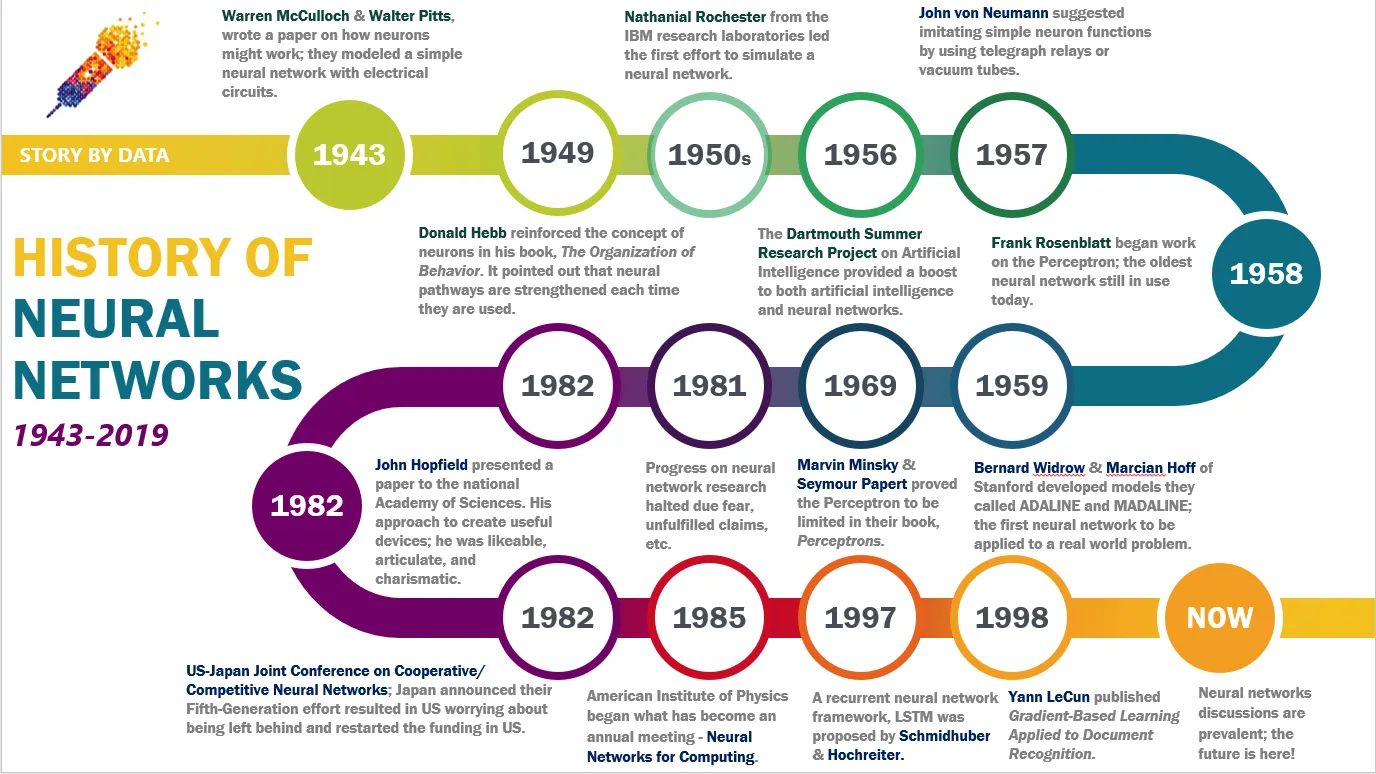
\includegraphics[width=1.15\textwidth]{images/Brief History of NN - Kate Strachnyi.png}
\end{frame}
%===============================================================================

%================================ 4 ============================================
\begin{frame}{The historical way...}
  \hspace*{-2mm}from: \href{https://pub.towardsai.net/a-brief-history-of-neural-nets-472107bc2c9c}
    {Pumalin: "A Brief History of Neural Nets", medium.com}\\[1mm]
  \hspace*{-8mm}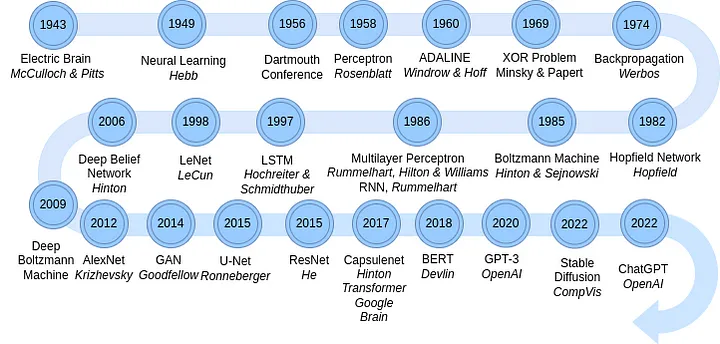
\includegraphics[width=1.15\textwidth]{images/A brief History of NN - Pumalin.png}
\end{frame}
%===============================================================================

%================================ 5 ============================================
\begin{frame}{The historical way...}
  \hspace*{-2mm}from: \href{https://towardsdatascience.com/ten-years-of-ai-in-review-85decdb2a540}
    {Thomas A Dorfe: "Ten Years of AI in Review", medium.com}\\[1mm]
  \hspace*{-6mm}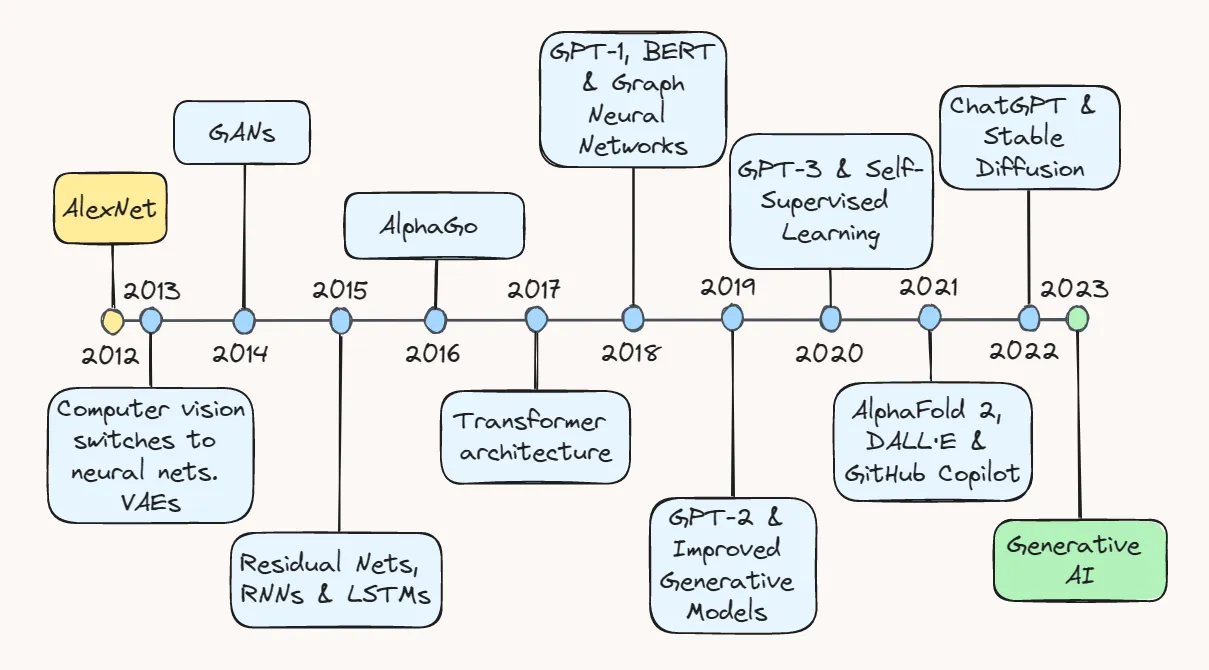
\includegraphics[width=1.1\textwidth]{images/Ten Years of AI in Review.png}
\end{frame}
%===============================================================================

%================================ 6 ============================================
\begin{frame}{Artificial Intelligence ?}

  \vspace*{-5mm}
  \begin {bclogo}[noborder=true, couleur=gray!50, couleurBarre=Chocolate, logo=\bctrombone, margeG=-0.8]
    {}
    \vspace*{-5mm}
    Historically\footnote{{\tiny first used in 1956 by \href{https://en.wikipedia.org/wiki/John\_McCarthy\_\%28computer\_scientist\%29}{John McCarthy},
    researcher at Stanford during the Dartmouth conference}} {\it badly chosen} term! Ambiguous current meaning...\\
    Many (contradictory) definitions depending on periods and authors...
    \end{bclogo}

  \visible<2->{

  \begin{itemize}
    {%\small
    \item {\em ''...the science of making computers do things that require intelligence when done by humans.}''
      {\tiny \href{http://www.alanturing.net/turing\_archive/pages/reference\%20articles/what\%20is\%20ai.html}{Alan Turing, 1940}}\smallskip
      
    \item {\em ''the field of study that gives computers the ability to learn without being explicitly programmed.''}
      {\tiny  \href{http://infolab.stanford.edu/pub/voy/museum/samuel.html}{Arthur Samuel, 1960}}\smallskip
      
    \item {\em ''A computer program is said to learn from experience E with respect to some class of tasks T and performance measure P,
      if its performance at tasks in T, as measured by P, improves with experience E.''}
      {\tiny \href{https://www.cs.cmu.edu/~tom/}{Tom Mitchell, 1997}}\smallskip
      
    \item Notion of {\em intelligent agent}, {\em rational agent} \\
      {\em ''...agent that acts in such a way as to reach the best solution or, in an uncertain environment, the best predictable solution.}''\\[-2mm]
      {\tiny  \href{http://aima.cs.berkeley.edu/translations.html}{Stuart Russel, Peter Norvig, ``Intelligence Artificielle'' 2015}}
    }
  \end{itemize}
  }
  
\end{frame}
%===============================================================================

%================================= 7 ===========================================
\begin{frame}{Artificial Intelligences ?}
 
  \textbf{Strong AI}

  \visible<1->{%
    \begin{itemize}
    \item Build systems that think exactly the same way that people do.
    \item Try also to explain how humans think... \Chocolate{Whe are not yet here}.
    \end{itemize}
  }

  \textbf{Weak AI}
  
  \visible<1->{% 
    \begin{itemize}
    \item Build systems that can behave like humans.
    \item The results will tell us nothing about how humans think.
    \item \Chocolate{We already are there}... We use it every day!\\
      (anti-spam, facial/voice recognition, language translation...)
    \end{itemize}
  }

  \visible<2->{%
  \textbf{General AI}
  \visible<1->{%
    \begin{itemize}
    \item AI systems designed for the ability to reason in general.
    \end{itemize}
  }

  \textbf{Narrow AI}
  \visible<1->{%
    \begin{itemize}
    \item AI systems designed for specific tasks.
    \end{itemize}
  }
  }
  
\end{frame}
%===============================================================================

\section{ML}

\subsection{ML Branches}

%================================== 8 ==========================================
\begin{frame}{Machine Learning: a field of AI}

  {\small Page from \href{https://medium.com/machine-learning-for-humans/why-machine-learning-matters-6164faf1df12}
  {medium.com/machine-learning-for-humans/...}}\\[2mm]
  
  \hspace*{-10mm}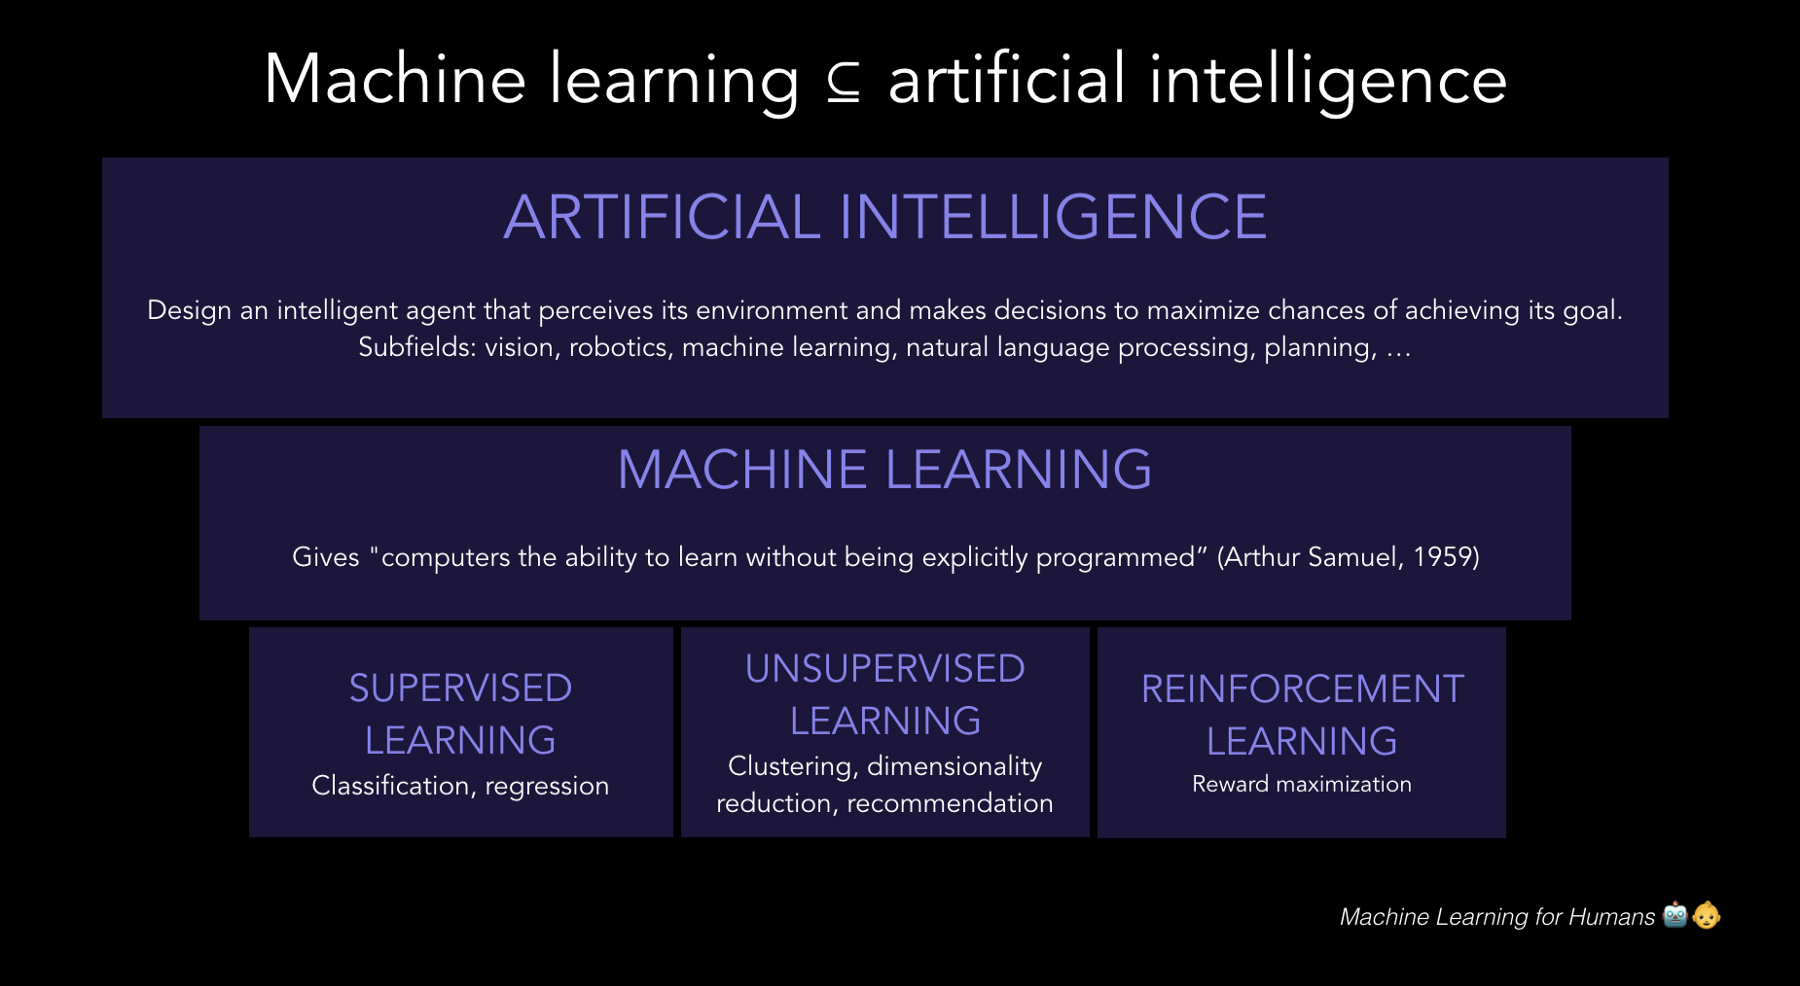
\includegraphics[width=1.2\textwidth]{images/AI-from_MachineLearningForHumans.png}
  \vspace*{-8mm}
  
\end{frame}
%===============================================================================

%================================== 9 ==========================================
\begin{frame}{Branches of Machine Learning}

  %% Excellent: https://www.ibm.com/cloud/learn/machine-learning?lnk=fle

  \begin{tcolorbox}[title={\bf Supervised learning}]
    {\bf labeled dataset} is used to train algorithms:
    \begin{itemize}
    \item \textbf{Classification}
      \begin{itemize}
      \item Images classification
      \item Objects detection in images
      \item Speech recognition...
      \end{itemize}
    \item \textbf{Regression}
      \begin{itemize}
      \item Predict a value...
      \end{itemize}
    \item \textbf{Anomaly detection}
      %% anomaliy detection with supervised laerning suppose that there are no "new annomaly" in the
      %% datat set to process, because the anomalies have been learned and the algorithm will not
      %% recognize new anomaly that was not learned...
      \begin{itemize}
      \item Spam detection
      \item Manufacturing: finding known (learned) defects
      \item Weather prediction
      \item Diseases classification...
      \end{itemize}        
    \end{itemize}
    \vspace*{-1mm}$\cdots$
  \end{tcolorbox}
  
\end{frame}
%===============================================================================

%=================================== 10 ========================================
\begin{frame}{Branches of Machine Learning}
  \begin{tcolorbox}[title={\bf Unsupervised learning}]
    Analyze and cluster \textbf{unlabeled datasets}:
    \begin{itemize}
    \item \textbf{Clustering} \& \textbf{Grouping} 
      \begin{itemize}
      \item Data mining, web data grouping, news grouping...
      \item Market segmentation
      \item Astronomical data analysis...
      \end{itemize}        
    \item \textbf{Anomaly Detection}
      \begin{itemize}
      \item Fraud detecion
      \item Manufacturing: finding defects even new ones
      \item Monitoring abnormal activity: failure, hacker, fraud...
      \item Fake account on Internet...
      \end{itemize}
    \item \textbf{Dimensionality reduction}
      \begin{itemize}
      \item Compress data using fewer numbers...
      \end{itemize}
    \end{itemize}
    \vspace*{-1mm}$\cdots$
  \end{tcolorbox}    
\end{frame}
%===============================================================================

%=================================== 11 ========================================
\begin{frame}{Branches of Machine Learning}  
  \begin{tcolorbox}[title={\bf Deep Reinforcement Learning} DRL]
    An agent (the Neural Network) learns how to drive an environment by maximising a \textbf{reward}:
    \begin{itemize}

    \item \textbf{Control/command}
      \begin{itemize}
      \item Controlling \href{run:./videos/trained-PPO-example.webm}{robots}, drones, \href{run:./videos/DRL-Cartpol.webm}{mecatronic systems}
      \item Factory optimization
      \item Financial (stock) trading...
      \end{itemize}        
    \item \textbf{Decision making}
      \begin{itemize}
      \item games (video games)
      \item financial analysis...
      \end{itemize}
    \end{itemize}
    \vspace*{-1mm}$\cdots$
  \end{tcolorbox}

  \begin{minipage}{\textwidth}
    \vspace*{-28mm}\hspace*{50mm}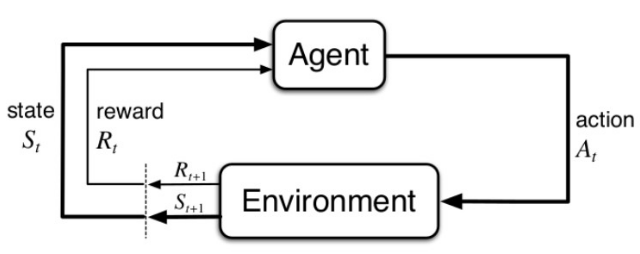
\includegraphics[width=.6\textwidth]{images/DRL.png}
  \end{minipage}

  \vfill
\end{frame}
%===============================================================================

\subsection{ML algorithms}

%=================================== 12 ========================================
\begin{frame}{}

  %See \href{https://www.ibm.com/cloud/learn/machine-learning}{www.ibm.com/cloud/learn/machine-learning}
  
  \begin{tcolorbox}[title=Various approaches for ML algorithms]
    {\small
      \begin{minipage}[t]{.55\textwidth}
        \bfdarkchoco{Supervised learning:}
        \begin{itemize}
        \item<1-> \only<1>{\Blue{Neural Networks}}\only<2>{\Blue{Neural Networks}}
        \item<1> Bayesian inference
        \item<1> Random forest
        \item<1> Decision Tree
        \item<1> Support Vector Machine (SVM)
        \item<1> K-Nearest Neighbor
        \item<1> Linear regression
        \item<1> Logistic regression
        \item<1>...
        \end{itemize}
      \end{minipage}\begin{minipage}[t]{.55\textwidth}
        \bfdarkchoco{Unsupervised learning:}
        \begin{itemize}
        \item<1-> \only<1>{\Blue{Neural Networks}}\only<2>{\Blue{Neural Networks}}
        \item<1> Principal Composant Analysis
        \item<1> Singular Value Decomposition
        \item<1> K-mean \& Prob. clustering
        \item<1>...
        \end{itemize}
        \medskip
        \bfdarkchoco{Reinforcement learning:}
        \begin{itemize}
        \item<1-> \only<1>{\Blue{Neural Networks} (Q-learning, Actor-Critic, DDPG, PPO...)}\only<2>{\Blue{Neural Networks}\\[5mm]} 
        \item<1> Monte Carlo
        \item<1> SARSA
        \item<1>...
        \end{itemize}
        
      \end{minipage}
    }
  \end{tcolorbox}    
  \visible<2->{This introduction deals only with \Blue{\bf Artificial Neural Networks}.}
\end{frame}
%===============================================================================

\subsection{Fields of ML}

%=================================== 13 ========================================
\begin{frame}{Fields \& applications of ML}

  \begin{tcolorbox}[height=6cm, add to width=.7cm, title=Computer Vision]
    \begin{minipage}[t][][t]{.6\textwidth}
      \begin{itemize}
      \item<1-> Image Classification
      \item<2-> Object Detection 
      \item<3-> (Semantic) Segmentation
      \item<4-> Image Generation\\
        {\small \href{https://www.leptidigital.fr/productivite/meilleurs-generateurs-images-ia-30857/}{Les 10 Meilleurs Générateurs d’Images}}
      \item<5-> Pose Estimation
      \item<5-> ...
      \end{itemize}
    \end{minipage}\begin{minipage}[t][][b]{.4\textwidth}
      \only<1>{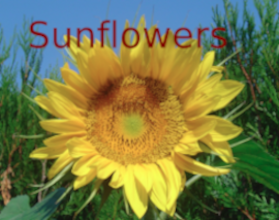
\includegraphics[width=1.\textwidth]{images/image_classification_sunflowers.png}}
      \only<2>{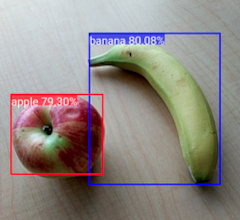
\includegraphics[width=1.\textwidth]{images/object_detection_aple-banana.png}\\[-2mm]
        {\centerline{\tiny Image credit: \href{https://www.tensorflow.org/lite/examples/object_detection/overview}{Tensorflow}}}}
      \only<3>{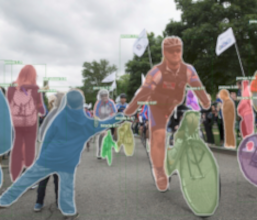
\includegraphics[width=1.\textwidth]{images/image_segmentation_Detectron.png}}
      \only<4>{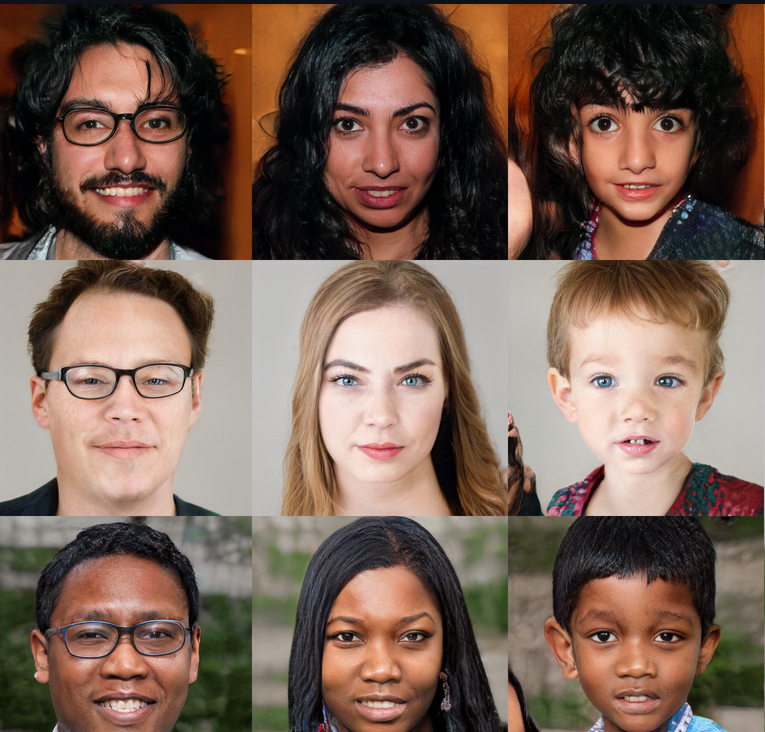
\includegraphics[width=1.\textwidth]{images/image_generation.png}\\[-2mm]
        {\centerline{\tiny Image credit: \href{https://github.com/NVlabs/stylegan}{stylegan}}}}
      \only<5>{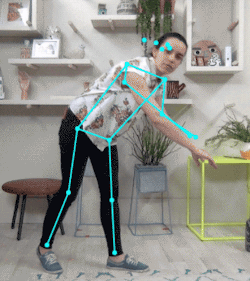
\includegraphics[width=1.\textwidth]{images/pose_estimation_TF.png}\\[-2mm]
        {\centerline{\tiny Image credit: \href{https://www.tensorflow.org/lite/examples/pose_estimation/overview}{Tensorflow-Pose Estimation}}}}
    \end{minipage}
  \end{tcolorbox}
  
\end{frame}
%===============================================================================

%=================================== 14 ========================================
\begin{frame}{Fields \& applications of ML}

  \begin{tcolorbox}[title=Natural Language Processing: NLP]
    \begin{itemize}
    \item<1-> Natural Language Understanding (NLU) 
    \item<1-> Natural Language Generation (NLG)
    \item<1-> Speech recognition / Speech Synthesis (Text To Speech)
    \item<1-> Machine Translation (languages)
    \item<1-> Virtual agents and ChatBots
    \item<1-> Optical character recognition (OCR)
    \item<1-> ...
    \end{itemize}
  \end{tcolorbox}   
  
\end{frame}
%===============================================================================

\subsection{Neural Networks achitectures}

%Physics-Informed Machine Learning Models

%=================================== 15 ==========================================
\begin{frame}{Neural Network Architectures}

Many NN architectures for many applications (non-exhaustive list):
\begin{itemize}
  \item \bfdarkchoco{Feed Forward}: the simplest architecture made of successive layers of neurones, with {\em Feed Forward} and {\em Back Propagation} algorithms.
  \item \bfdarkchoco{Convolutional} (CNN): Mostly used for analyzing and classifying images.
  \item \bfdarkchoco{Recurrent} (RNN): Used for time series, like the Long Short-Term Memory (LSTM) algorithm.
  \item \bfdarkchoco{Transformers} : Recently used for Natural Language Processing and then for image classification.
  \item \bfdarkchoco{Auto Encoder} (AEN): Dimensionality reduction, Feature extraction, Denoising of data/images, Inputing missing data.
  \item \bfdarkchoco{Generative Adversarial} (GAN): to generate text, images, music...
  \item \bfdarkchoco{Large Language Model} (LLM): read text, sound, write books, images, speak, make music ...ChatGPT
\end{itemize}
{\small\centering[Synthetic Graphical chart: \href{https://chart-studio.plotly.com/~SolClover/90.embed?autosize=true&referrer=https\%3A\%2F\%2Ftowardsdatascience.com\%2F}{from Saul Dobilas on Medium}] }
\end{frame}
%===============================================================================

\section{societal issues}

\subsection{Explainability}

%=================================== 16 ==========================================
\begin{frame}{Societal issues: {\bf Explainabilty}}

  \DarkGreen{\bf Explainability} is fast becoming a top priority in research, where it is often
  abbreviated as \\
  \hspace*{10mm}{\bf xAI} \hspace*{10mm}{\bf Explainable} Artificial Intelligence\\
  \hspace*{10mm}{\bf iML} \hspace*{10mm}{\bf Interpretable} Machine learning
  \bigskip

  \begin{tcolorbox}[title={\bf Explainability}]
    \begin{itemize}
    \item {\bf Unexplainability} of the results computed by Neural Networks still constitutes an obstacle to their dissemination today.
    \item Deep learning with Neural Networks is often denigrated as a {\bf Black box} by scientists with a Cartesian approach.
    \item Even ML developpers have difficulties to explain by which way a NN decision has been computed
    \end{itemize}
  \end{tcolorbox}   
    
  
\end{frame}
%===============================================================================

\subsection{decision-making}

%=================================== 17 ==========================================
\begin{frame}{Societal issues: {\bf Decision-making ML}}

  An increasing amount of {\bf decisions} in sensible fields are being ceded to ML algorithms to the detriment of
  human control, raising concern for loss of fairness and equitability.
  
  \begin{tcolorbox}[title={\bf Explainability}]
    \begin{itemize}
    \item  Decision-making algorithms rest inevitably on assumptions, even silent ones, such as the quality of data the algorithm is trained
    \item 
    \end{itemize}
  \end{tcolorbox}   
  
  Machine-learning algorithms in the field of criminal justice

  Certification....
  
\end{frame}
%===============================================================================

\subsection{trustworthy AI}

%=================================== 18 ==========================================
\begin{frame}{Societal issues: {\bf Trustworthy AI}}

  \hspace*{-2mm}\begin{minipage}{.35\textwidth}
    
\includegraphics[width=\linewidth]{images/logo-ec--en.png}
  \end{minipage}\ \begin{minipage}{.65\textwidth}
  \small
    On 8 April 2019, the High-Level Expert Group on AI presented
  \href{https://digital-strategy.ec.europa.eu/en/library/ethics-guidelines-trustworthy-ai}
       {Ethics Guidelines for Trustworthy Artificial Intelligence}
  \end{minipage}
\bigskip      
  \begin{tcolorbox}[title={According to the Guidelines, trustworthy AI should be:}]   
    
    \begin{description}
    \item[\DarkBlue{Lawful}]  respecting all applicable laws and regulations
    \item[\DarkBlue{Ethical}] respecting ethical principles and values
    \item[\DarkBlue{Robust}] both from a technical perspective while taking into account its social environment       
    \end{description}
  \end{tcolorbox}   
       
\end{frame}
%===============================================================================

%=================================== 19 ==========================================
\begin{frame}{Societal issues: Trustworthy AI}

  \hspace*{-5mm}
  \begin{minipage}{.5\textwidth}
    {\Large\bf ALTAI}\\
    Assessment List for Trustworthy AI
  \begin{itemize}
  \item Does the AI system potentially negatively discriminate against people...?
  \item Does the AI system respect the rights of the child?
  \item Does the AI system protect personal data relating to individuals in line with GDPR?
  \item Does the AI system respect the freedom of expression and information and/or freedom of
    assembly and association?
  \end{itemize}
  \end{minipage}\begin{minipage}{1.\textwidth}
   \hspace*{2mm}\vspace*{-2mm}
  
\includegraphics[width=.6\textwidth]{images/ALTAI.png}
  \end{minipage}
  
\end{frame}
%===============================================================================


%=================================== 18 ==========================================
\begin{frame}{Some societal issues}

  References
  \begin{itemize}
  \item The Alan Turing Institute\\
    \href{http://arxiv.org/abs/1906.05684}{Understanding artificial intelligence ethics and safety}
  \item Nature\\
    \href{https://www.nature.com/articles/s41599-020-0501-9}{Ethical principles in machine learning and artificial intelligence: cases from the field and possible ways forward}
  \end{itemize}

\end{frame}
%===============================================================================

\section{Internet resources}

https://towardsdatascience.com/


\section{Computing aspects}

\subsection{The artificial neuron}

%================================== 21 =========================================
\begin{frame}{Computing aspects}
  
  \tikzset{%
  neuron/.style={
    circle,
    draw,
    minimum size=1cm,
    font=\large
  },
  squa/.style={
    draw,
    inner sep=2pt,
    font=\large,
    join = by -latex
  },
  }
  \begin{tcolorbox}[title=The Artificial neuron model]  
    %\hspace*{-.7cm}
    \begin{tikzpicture}[x=1.4cm, y=1.cm]

      \node [label=above:\parbox{2cm}{\centering Input\\stimuli}] at (0, 1.5) (x1)  {$x_1$};
      \node [] at (0, 0.5) (x2) {$x_2$};
      \node [] at (0, -0) (vdots) {$\vdots$};
      \node [] at (0, -0.7) (xn) {$x_n$};
      \node [label=above:\parbox{2cm}{\centering Bias}] at (2, 2) (bias) {$b$};
      \node [label=above:\parbox{2cm}{\centering Output}] at (4, 0.15) (y) {$y = f(\sum_i{w_{i}\,x_i} - b)$};
      
      \node [neuron/.try] (output) at (2,0.15) {\large{$\displaystyle{\Sigma | f}$}};
      
      \draw [o-latex] (x1) -- (output);
      \draw [o-latex] (x2) -- (output);
      \draw [o-latex] (xn) -- (output);
      \draw [o-latex] (bias) -- (output);
      \draw [->] (output) -- (y);

      \node [] at (1,1) () {$w_1$} ;
      \node [] at (1,.5) () {$w_2$} ;
      \node [] at (1, -0.45) () {$w_n$} ;
    \end{tikzpicture}
  \end{tcolorbox}
  \smallskip
  \visible<1->{An \bfdarkchoco{artificial neuron}:
    \begin{itemize}
    \item <1-> receives the input stimuli $(x_{i})_{i=1..n}$ with \textbf{weights} $(w_i)$
    \item <1-> computes the \textbf{weighted sum} of the input $\sum_i{w_{i}\,x_i - b}$
    \item <1-> outputs its activation $f(\sum_i{w_{i}\,x_i} - b)$, computed with a non-linear \textbf{activation function} $f$ .
    \end{itemize}
  }

\end{frame}
%===============================================================================

\subsection{Activation functions}

%================================= 22 ==========================================
\begin{frame}{Computing aspects}
  
  \begin{tcolorbox}[add to width=.7cm, title={Common activation functions}]
    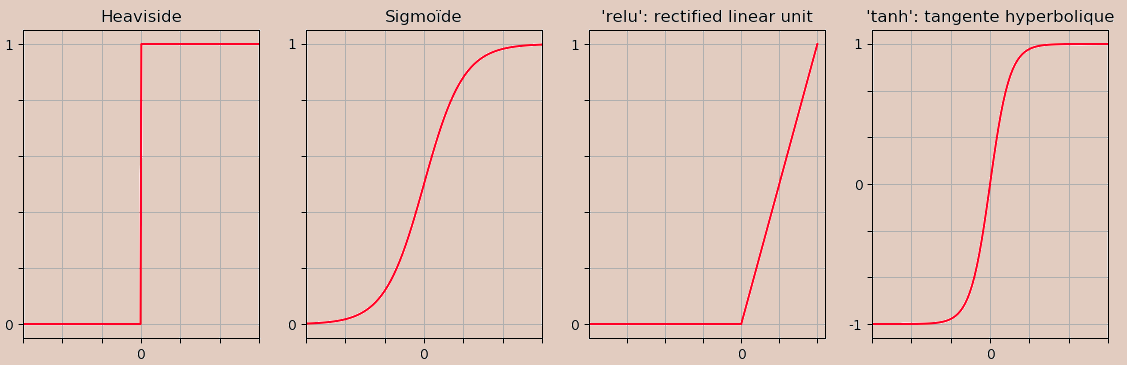
\includegraphics[width=1.\textwidth]{images/activ_functions-2.png}
  \end{tcolorbox}
  
  \begin{itemize}
  \item Introduces a non-linear behavior.
  \item Sets the range of the neuron output: $[-1, 1]$, $[0, 1]$, $[0, \infty[$...
    \item The bias $b$ sets the activation threshold of the neuron.
  \end{itemize}
  
\end{frame}
%===============================================================================

\subsection{Activation functions SoftMax}

%================================== 23 =========================================
\begin{frame}{Computing aspects}
  \vspace*{-2mm}

  \begin{itemize}
    
  \item intermediate layers $\leadsto$ \bfdarkchoco{relu} promotes network learning
    \footnote{{\tiny avoids the {\em vanishing gradient} that appears in {\em back propagation}}}.\smallskip
    
  \item \bfdarkchoco{softmax} always used for in the last layer for {\bf Classifying}.
    
  \end{itemize}
  \smallskip
  
  \begin{tcolorbox}[add to width=.7cm, title={Example: ativation function {\em softmax} for the last layer, 10 classes}]
    
    \begin{minipage}{.55\textwidth}
      \vspace*{-2mm}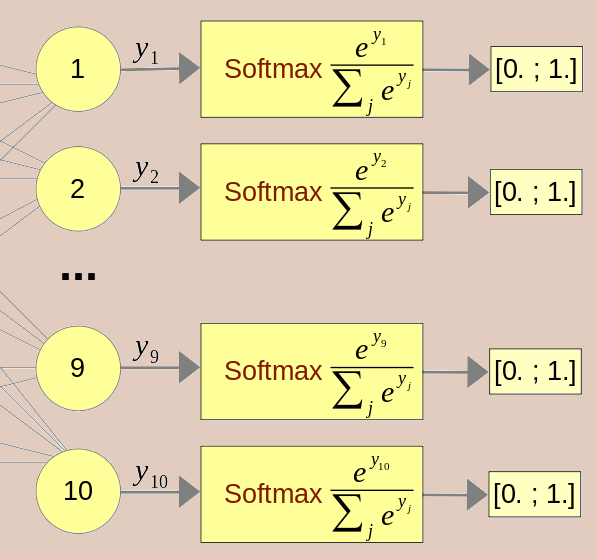
\includegraphics[width=0.8\textwidth]{images/softmax-2.png}
    \end{minipage}\hspace*{5mm}\begin{minipage}{.45\textwidth}
      {\small
        \begin{itemize}
        \item The activation of neuron $k$ is $Y_k = e^{y_k}/\sum_i{e^{y_i}}$
          with $y_k = \sum_i \omega_i x_i - b$ calculated by the neuron $k$.
        \item The neurons outputs are interpreted as {\bf probabilities} in the interval [0,1].
        \item[\Black{$\leadsto$}] <2> the label of the neuron with the highest probability is the network response
      \end{itemize}}
    \end{minipage}
  \end{tcolorbox}
    
\end{frame}
%===============================================================================

\subsection{One-hot coding}

%================================= 24 ==========================================
\begin{frame}{Computing aspects [Classitication]}

\begin{tcolorbox}[title={\em One-hot} coding of labels]

     Goal: transform the image labels to match the network output (vector of probabiliies):

     {\small
       \begin{itemize}
       \item Image labels: ordered set \textbf{integers}.
       \item Network output: \textbf{vector of \texttt{float}} in the interval [0;1] calculated by the {\em softmax} activation of the output neurons.
       \item {\em One-hot} coding of an ordered set $\mathfrak{L}$ of $N$ labels: \\[1mm]
         - each label value is coded as a vector with $N$ components all zero except one (equal to $1$),\\
         - the rank of the $1$ in the vector gives the value of the labe.
       \end{itemize}
     }
\end{tcolorbox}

\visible<2>{
  \begin{minipage}{.3\textwidth}
    \vspace*{-22mm}\hspace*{-5mm}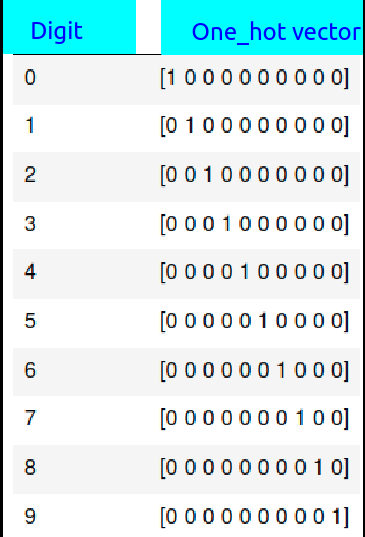
\includegraphics[width=1.1\textwidth]{images/oneHotCoded.png}
  \end{minipage}
  \begin{minipage}{.6\textwidth}
    \vspace*{-5mm}{\small The {\em one-hot} encoding of the labels '0' to '9' gives a vector with 10 components.}
  \end{minipage}
}
    
\end{frame}
%===============================================================================

%================================== 25 =========================================
\begin{frame}{Computing aspects [Classitication]}

\begin{tcolorbox}[title=Error function: {\em Cross entropy error}]

  \begin{itemize}
  \item The image analysed by the network $\leadsto$ vector $\hat{Y}$ of \texttt{float} to be compared to the vector $Y$ of the {\em hot-one} encoding of the true image label.
  \item The error (loss) function {\em cross entropy} is adapted to {\em one-hot} coding: $e(Y,\hat{Y})=-\sum_i Y_i\ log(\hat {Y}_i)$\\
    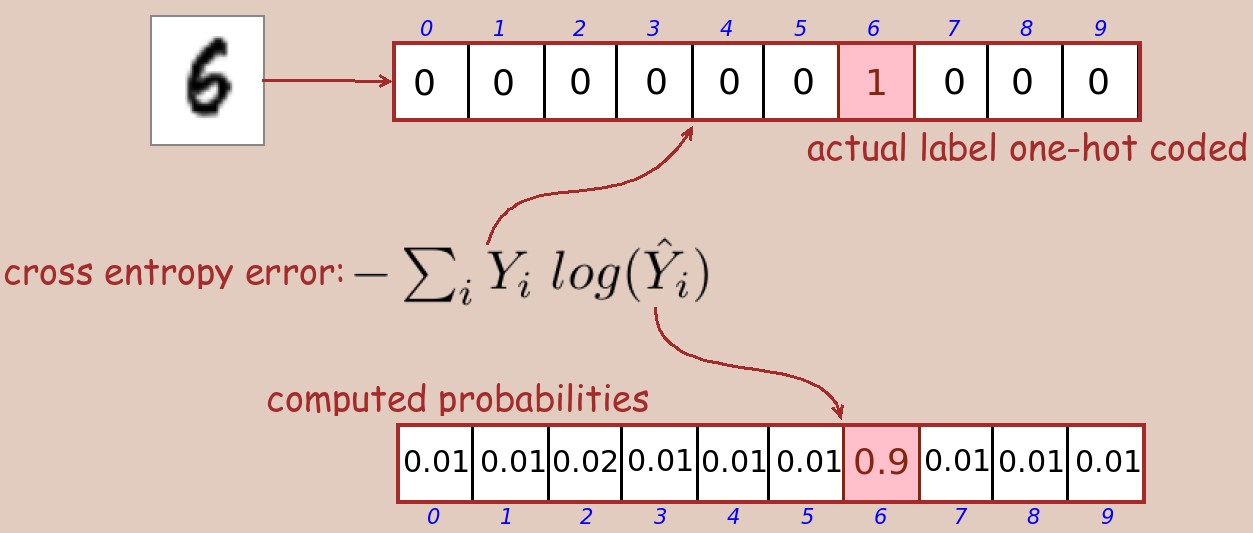
\includegraphics[width=.9\textwidth]{images/CrossEntropyError.png}
  \end{itemize}
  
   \end{tcolorbox}  
\end{frame}
%===============================================================================

\subsection{Optimisation}

%=================================== 26 ========================================
\begin{frame}{Computing aspects}

\begin{tcolorbox}[title=Optimization and {\em Back Propagation}]

  \begin{itemize}
    \visible<1->{\item During the training an optimization algorithm computes the gradient of the error function
      with respect to the network weights.}
    \visible<2->{\item The {\em Back Propagation} algorithm \textbf{modifies} the weights of the network layer by layer thanks to the gradient of the error function,
      iterating from the last layer to the first layer. }
    \visible<3->{\item Examples of optimization algorithms:
      \begin{itemize}
      \item Gradient Descent ({\em Gradient Descent (GD)})
      \item Stochastic Gradient Descent ({\em Stochastic Gradient Descent (SGD)})
      \item {\em \href{https://arxiv.org/abs/1412.6980}{Adam}} (improved version of gradient descent)...
      \end{itemize}

      {\small The module \href{https://www.tensorflow.org/api_docs/python/tf/keras/optimizers}{tf.keras.optimizers}
        provides Python implementation of several optimization algorithms.}}
      
  \end{itemize}
\end{tcolorbox}

\end{frame}
%===============================================================================

\subsection{Back-propgation algorithm}

%==================================== 27 =======================================
\begin{frame}{Computing aspects}

  {\small Visualization of iterations of gradient descent algorithms for an very-simple loss function with only 2 variables:}\\[2mm]
  \hspace*{25mm}\href{https://github.com/Jaewan-Yun/optimizer-visualization/blob/master/figures/movie9.gif}{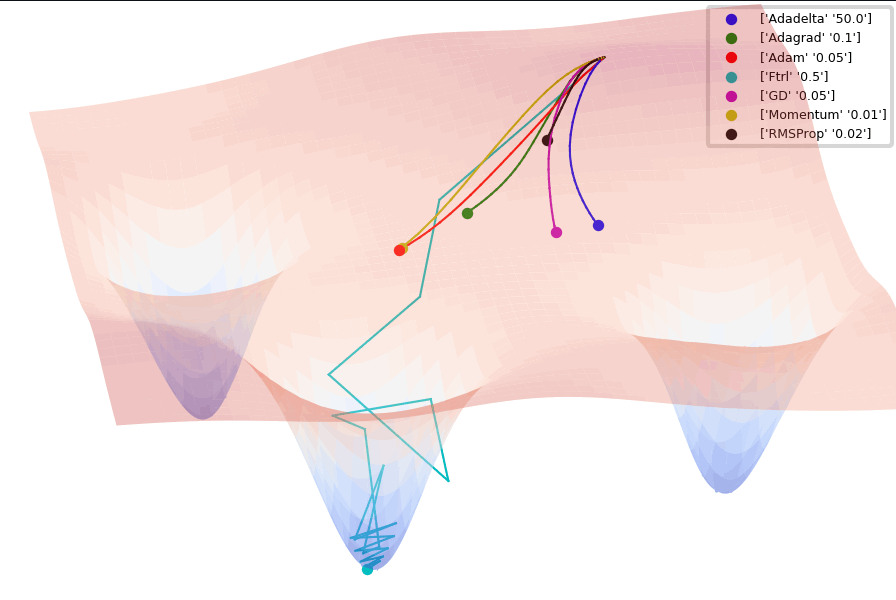
\includegraphics[width=.45\textwidth]{images/adam_plot3D_animated.png}}\\[-2mm]
  %\hspace*{8mm}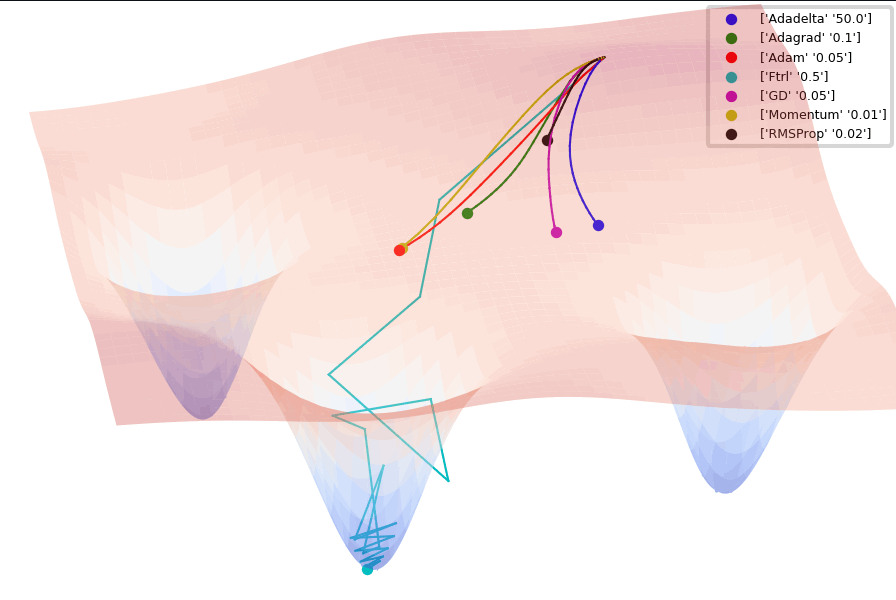
\includegraphics[width=.8\textwidth]{images/adam_plot3D_animated.png}\\[-2mm]
  %\animategraphics[width=.8\textwidth,controls]{10}{./images/Adam-plot3D/movie9/img_}{0}{114}
  \hspace*{25mm}{\tiny (source: \href{https://github.com/Jaewan-Yun/optimizer-visualization}{github.com/Jaewan-Yun/optimizer-visualization})}
  
  \medskip
      {\small Video explaining the {\em back propagation} algorithm:}\\
      \hspace*{30mm}\href{https://www.3blue1brown.com/lessons/backpropagation}{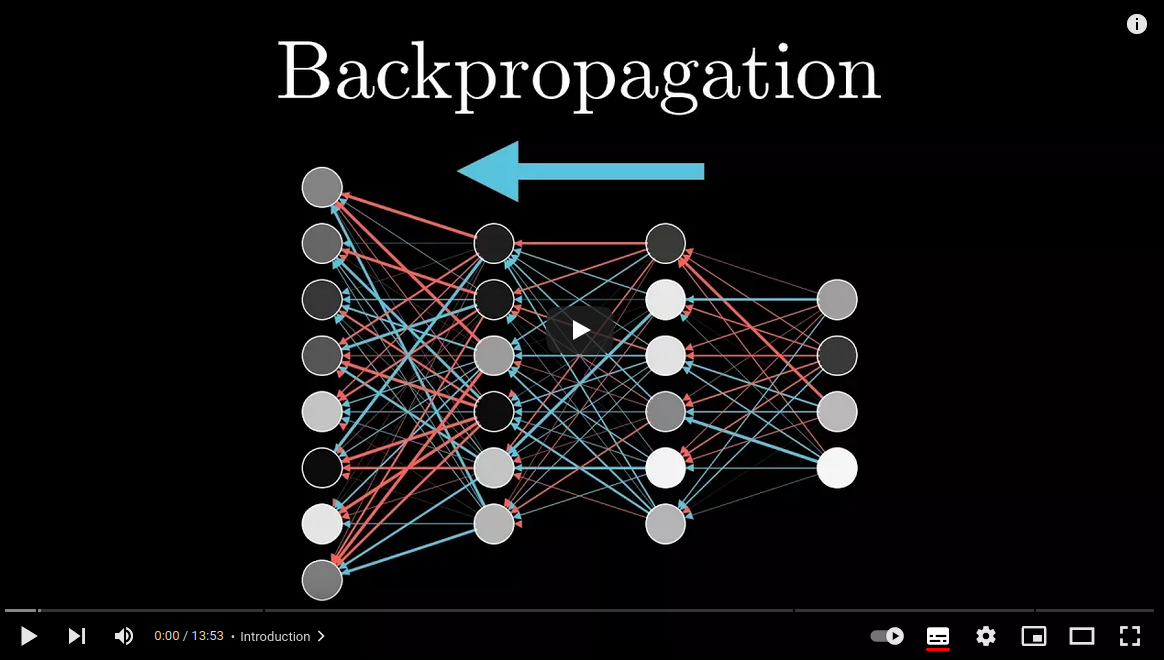
\includegraphics[width=.35\textwidth]{images/video-BackPropagation.png}}
\end{frame}
%===============================================================================

\subsection{Supervised learning}

%================================== 28 =========================================
\begin{frame}{Computing aspects}

  {\small
    \vspace*{-1mm}\hspace*{-10mm}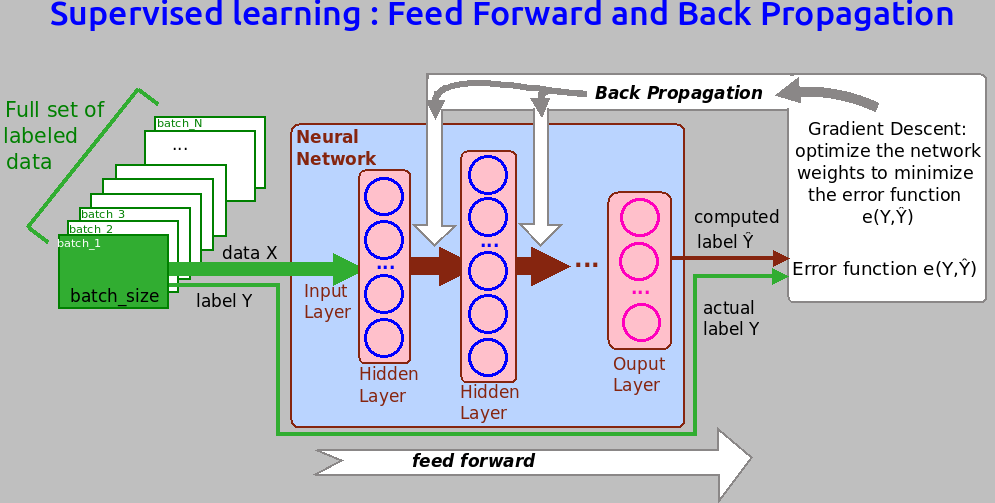
\includegraphics[width=1.18\textwidth]{./images/NetworkTraining.png}
  \vspace*{-4mm}\begin{itemize}
  \item The dataset is split into (mini) {\bf batches} of size \code{batch\_size}
  \item After each {\em feed forward} the {\em Back Propagation} algorithm modifies the weights
    neurons to minimize the error $e$.
  \end{itemize}
  }
\end{frame}
%===============================================================================

\subsection{Supervised learning}

%================================= 29 ==========================================
\begin{frame}{Computing aspects}

  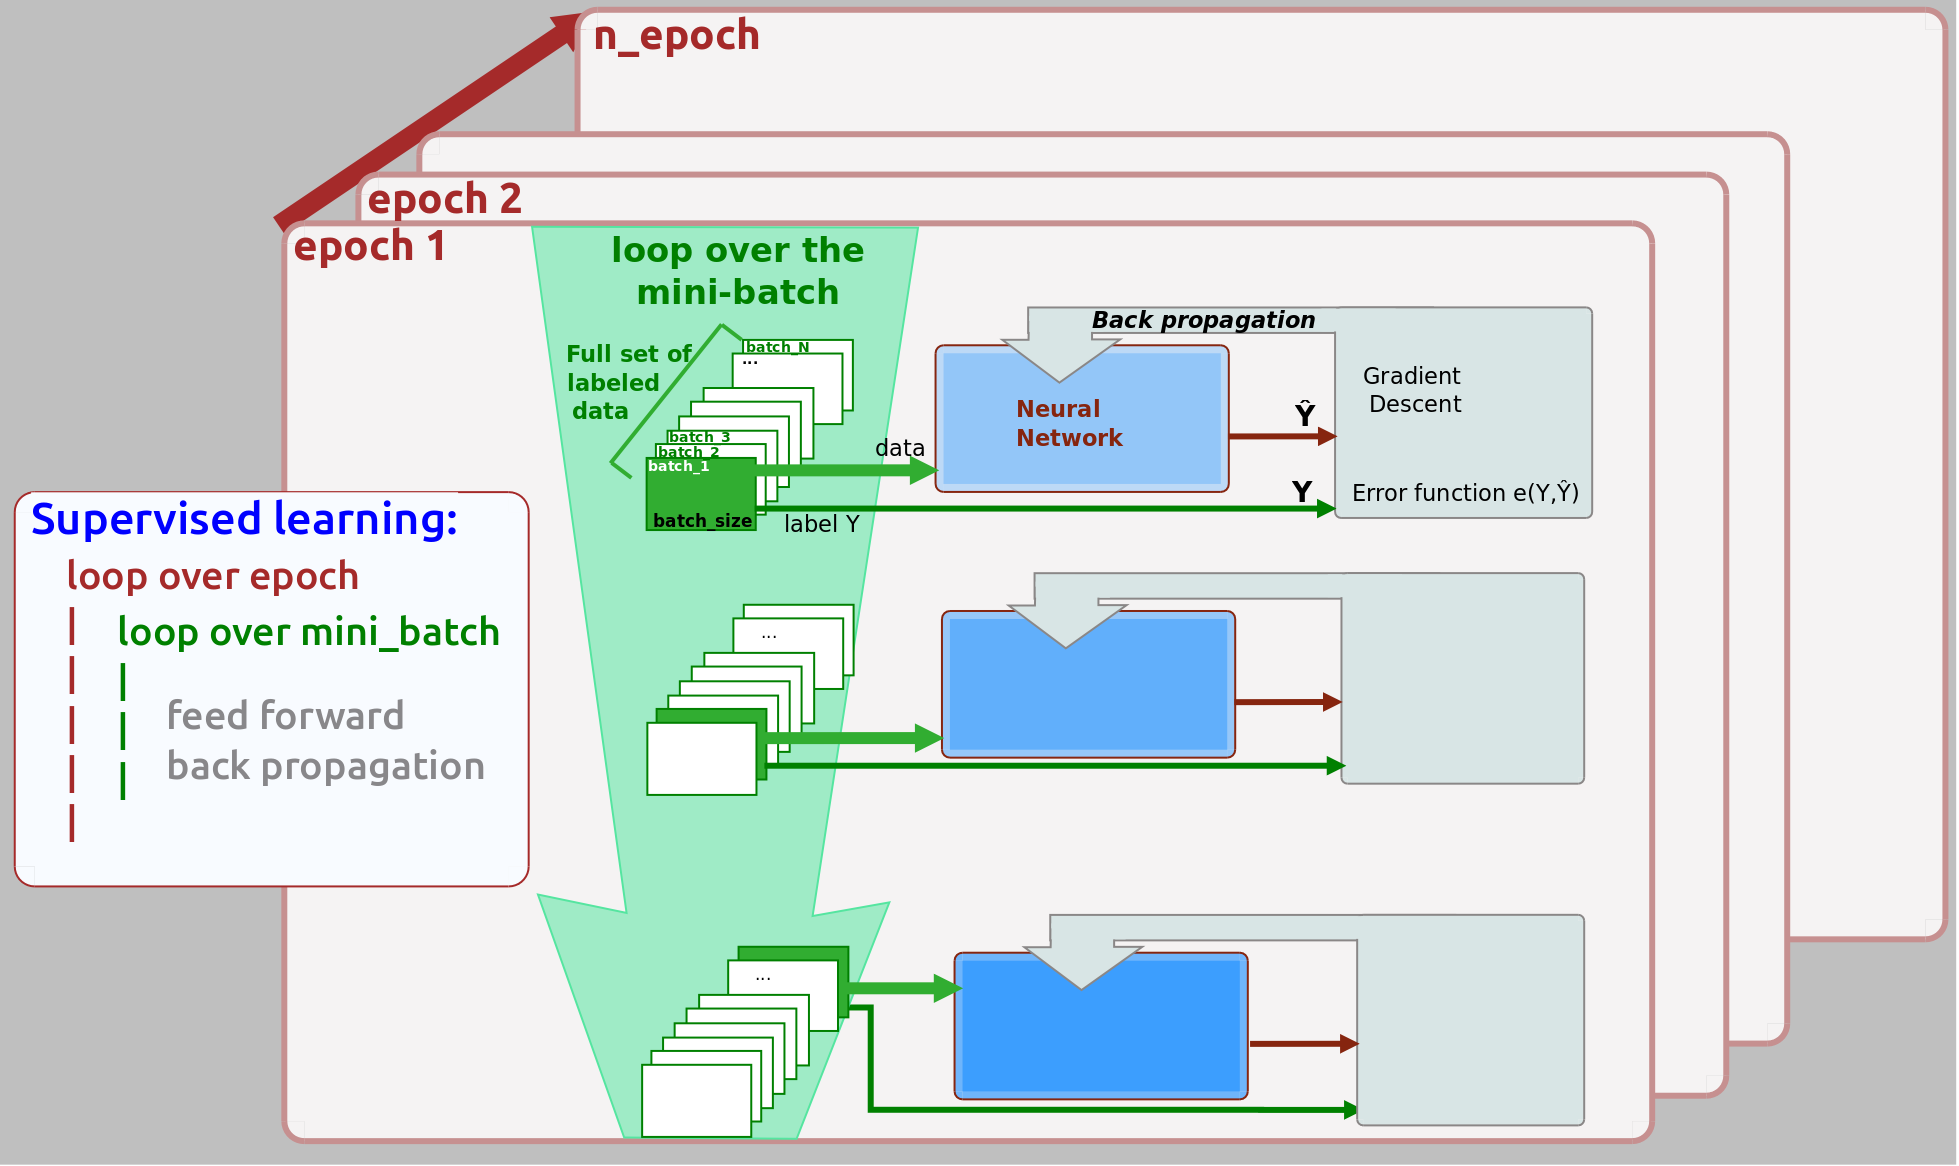
\includegraphics[width=\textwidth]{./images/NetworkTraining_2.png}
  \vspace*{-3mm}\begin{itemize}
  \item Training with the whole dataset is repeated \code{n\_epoch} times,
  \item The network state at the end of epoch \code{n} becomes the initial state for epoch \code{n+1}.
   \end{itemize}  
\end{frame}
%===============================================================================

\section{PVE}

\subsection{Motivation}

%=================================== 16 ========================================
\begin{frame}{Why use PVE to develop ML programs with Python}

  \visible<1->{
  \begin{tcolorbox}[title=PVE Advantages]
    \begin{itemize}
    \item To create a dedicated environment (disk tree) with fixed version of the Python interpreter and sensitive modules (like tensorflow)
    \item Easy to create and destroy as many times as you want
    \item To Protect your projects against operating system updates or hazardous manipulations...\\
      \visible<1->{
        $\leadsto$ \DarkGreen{you can load/update modules within a PVE without breaking\\\phantom{$\leadsto$ }modules compatibility for the other projects}
        }
    \item Each Python project should have its own PVE...
    \end{itemize}
  \end{tcolorbox}
  }
  \visible<1->{
    \bigskip
  \begin{tcolorbox}[title=Disadvantages]
    \begin{itemize}
    \item ? (just do it)
    \end{itemize}
  \end{tcolorbox}
  }

\end{frame}
%===============================================================================
 
\end{document}


%=================================== 17 ========================================
\begin{frame}{PVE: simple to create \& use}
  
  \begin{tcolorbox}[add to width=.7cm, title=Create/populate a PVE with {\bf conda}]
    \begin{itemize}
    \item <1-> Download \& install \href{https://docs.conda.io/en/latest/miniconda.html}{miniconda} for your OS.
    \item <2-> \code{\$ conda create -n dumas1 python=3.8} $\leadsto$ {\small creates the \DarkRed{\boldtt{dumas1}} PVE}
    \item <3-> \code{\$ conda activate dumas1} $\leadsto$ {\small activates the \DarkRed{\boldtt{dumas1}} PVE }
    \item <4-> \code{\$ conda env update -n dumas1 --file <file.yml>} $\leadsto$ {\small loads all the Python modules listed in \file{file.yml} into the \DarkRed{\boldtt{dumas1}} PVE }
    \item <5-> {\small\bf Use with caution}: \code{\$ conda install <module>} or \code{\$ pip install <module>} {\small $\leadsto$ adds a module to the {\bf activated} \DarkRed{\boldtt{dumas}} PVE.}
    \end{itemize}
  \end{tcolorbox}    

  \visible<6->{\small
  \begin{tcolorbox}[add to width=.7cm, title=Advantages / disadvantages]
    \begin{itemize}
    \item[\happy] <6-> The version of Python in a conda PVE can be $\neq$ version of the interpreter that comes with the OS installation
    \item[\happy] <7-> Some modules installed with \Chocolate{conda} can be more performant\\
      $\leadsto$ numpy \& tensorflow are linked with the \href{https://www.intel.com/content/www/us/en/developer/tools/oneapi/onemkl.html}{MKL} library\\[1mm]
    \item[\unhappy] <8->\Chocolate{conda install} and \Chocolate{pip install} can be conflicting...
    \end{itemize}
  \end{tcolorbox}
  }
  
\end{frame}
%===============================================================================

%=================================== 18 ========================================
\begin{frame}{PVE: simple to create \& use}
  
  \begin{tcolorbox}[add to width=.7cm, title=Create/populate a PVE with {\bf venv}]
    
    \begin{itemize}
    \item <1-> \code{\$ pip install venv} $\leadsto$ {\small Installs the \href{https://docs.python.org/3/library/venv.html}{venv} Python module}
    \item <2-> \code{\$ python -m venv dumas1} $\leadsto$ {\small creates the PVE named \DarkRed{\boldtt{dumas1}}}
    \item <3-> \code{\$ source ./dumas1/bin/activate} $\leadsto$ {\small activates the \DarkRed{\boldtt{dumas1}} PVE }
    \item <4-> \code{\$ pip install -r <requirements.txt>} $\leadsto$ {\small loads all the Python modules listed in \file{requiremnts.txt} into the \DarkRed{\boldtt{dumas1}} PVE }
    \item <5-> \code{(dumas1) \$ pip install <module>}\\
      $\leadsto$ {\small installs a module for the {\bf activated} \DarkRed{\boldtt{dumas1}} PVE}\\
      $\leadsto$ {\small note the path prefix \code{(dumas1)} showing the activated PVE}
    \end{itemize}
    
  \end{tcolorbox}    

  
  \visible<6->{\small
  \begin{tcolorbox}[add to width=.7cm, title=Advantages / disadvantages]
    \begin{itemize}
    \item[\unhappy] <6-> The version of Python for the PVE is the version of the interpreter that comes with the OS installation
    \item[\happy] <7-> No conflict with \Chocolate{conda install}
    \end{itemize}
  \end{tcolorbox}
  }
\end{frame}
%===============================================================================

%=================================== 19 ========================================
\begin{frame}[fragile]{Installation of Python modules}

\hspace*{-5mm}Examples of files for the \DarkRed{\boldtt{dumas1}} PVE:\\[-5mm]

  \hspace*{5mm}\begin{minipage}[t]{.35\linewidth}
    \begin {bclogo}[noborder=true, couleur=gray!50, couleurBarre=Chocolate, logo=\bctrombone, marge=0, margeG=-.8]
    {{\small YAML format for} \codeBF{conda}}
    \begin{minted}[frame=single, fontsize=\footnotesize]{yaml}
name: dumas1
channels:
  - defaults
dependencies:
  - python=3.8
  - tensorflow==2.8.*
  - pandas
  - matplotlib
  - opencv
  - jupyter
  - notebook
  - scikit-learn
  - seaborn
  - pip
\end{minted}
    \end{bclogo}
  \end{minipage}
\hspace*{25mm}\begin{minipage}[t]{.3\linewidth}
    \begin {bclogo}[noborder=true, couleur=gray!50, couleurBarre=Chocolate, logo=\bctrombone, marge=0, margeG=-.8]
    {{\small TXT format for} \codeBF{pip}}
\begin{minted}[frame=single, fontsize=\footnotesize]{text}
tensorflow==2.8.*
pandas
matplotlib
opencv-python
jupyter
notebook
scikit-learn
seaborn
\end{minted}
    \end{bclogo}
    \end{minipage}  

\end{frame}
%===============================================================================
%=================================== 20 ========================================
\begin{frame}{PVE: simple to create \& use}
  
  \begin{tcolorbox}[title=the winning recipe]
    
    \begin{itemize}
    \item <1-> One \Chocolate{PVE} for every ML project
    \item <2-> \Chocolate{Git} repository (GitHub, GitLab...) for storing, sharing \& versionning the project files
    \item <3-> \file{myfile.yml} to install the Python modules for the \codeBF{conda} PVE of each project, or
      \file{myfile.txt} for a \codeBF{pip} PVE.
    \item <4-> \Chocolate{Jupyter notebook} and/or \Chocolate{Visual studio code} ({\it aka} VSCode) to developp Python programs.
    \item[\happy] <5-> Like many IDEs \Chocolate{VSCode} is aware of PVEs.
      
    \end{itemize}
  \end{tcolorbox} 
\end{frame}
%===============================================================================



================================================================================

\section{Reproducibility of training}

\subsection{Motivation}

%=================================== nn ========================================
\begin{frame}{Reproducibility of training}
  
  \begin{tcolorbox}[title=Where to find randomness in NN training]
    
    \begin{itemize}
    \item<1-> \bfdarkchoco{Random initialization of the weights} of the network before the training starts.
    \item<2-> Regularization, e.g. {\bf dropout}, which involves randomly dropping nodes in the network while training.
    \item<3-> Optimization process like {\bf stochastic gradient descent} or {\bf Adam} also include randomness.
    \item<4-> Shuffling of data to build batches to train the NN
    \item<5-> and many others stages in ML algorithms  where random genertaors are used...
    \end{itemize}
  \end{tcolorbox}
    
\end{frame}
%===============================================================================
 
\subsection{Practical work with tensorflow}

%=================================== nn ========================================
\begin{frame}{Reproducibility of training}
  
  \begin{tcolorbox}[title=Practical work with tensorflow]
    
    \begin{itemize}
    \item<1-> We will run a \bfdarkchoco{Jupyter notebook} to illustrate the {\it Reproducibility of training} with {\bf tensorflow}.
    \item<2-> See the PVE usage
    \item<3-> Create a simple {\it Feed Forward} dense network and train it to classify {\it hand written} images form the MNIST
    \item<4-> Explore where and how the question of the Reproducibility occurs... and how to solve it \dSmiley[1.][green!60!white]
    \end{itemize}
  \end{tcolorbox}

    
\end{frame}
%===============================================================================
 
\subsection{References}

%===============================================================================
\begin{frame}{}
  
  \noindent\fontsize{8}{8}\selectfont{

    \hspace*{-4mm}\hypertarget{refRusselNorvig}{[1] }%
    {\em Artificial Intelligence: A Modern Approach (4th Edition)}, By Stuart Russell \& Peter Norvig. 
    Pearson, 2020. ISBN 978-0134610993. \href{http://aima.cs.berkeley.edu/}{aima.cs.berkeley.edu}\\[3mm]
    {\em Intelligence artificielle -- Une approche moderne -- 4e éd.}, By Stuart Russell \& Peter Norvig. 
    Translated by L. Miclet, F. Popineau, \& C. Cadet. Paris: Pearson Education France, 2021. ISBN 978-2326002210.\\[5mm]


    \hspace*{-4mm}\hypertarget{refStrongWeak-AI}{[2] }%
    {\em What is artificial intelligence (AI), and what is the difference between general AI and narrow AI?}, Kris Hammond, 2015\\
    \href{https://www.computerworld.com/article/2906336/what-is-artificial-intelligence.html}
         {www.computerworld.com/article/2906336/what-is-artificial-intelligence.html}\\[5mm]

    \hspace*{-4mm}\hypertarget{StanfordEncyc}{[3] }%
    {\em Stanford Encyclopedia of Philosophy},
    \href{https://plato.stanford.edu/entries/artificial-intelligence}
         {plato.stanford.edu/entries/artificial-intelligence}\\[5mm]

    \hspace*{-4mm}\hypertarget{DeepLeraning}{[4] }%
    {\em  Deep Learning.}, Goodfellow, Ian; Bengio, Yoshua; Courville, Aaron (2016), MIT Pres, ISBN 9780262035613
  }
  
\end{frame}
%===============================================================================
